\documentclass[a4paper,fleqn]{cas-dc}
\usepackage[numbers,sort&compress]{natbib}
\usepackage{tabularx,longtable,adjustbox,placeins}
\usepackage{lmodern,microtype}
\hypersetup{hidelinks}
\setlength{\emergencystretch}{1em}
\graphicspath{{figures/}}
\newcommand{\ind}{\mathbf{1}}
\begin{document}
\let\WriteBookmarks\relax
\shorttitle{Deadline-Limited Communication in MARL}
\shortauthors{Kung and Ha}
\title[mode=title]{Evaluating Deadline-Limited Communication in Multi-Agent Reinforcement Learning: Delivery, Computation, and Control}
\author[1]{Yeong-woo Kung}
\author[1]{Young-guk Ha}
\cormark[1]
\affiliation[1]{organization={Smart Computing Laboratory, Department of Computer Science \& Engineering, Konkuk University},
  city={Seoul}, postcode={05029}, country={Republic of Korea}}
\cortext[1]{Corresponding author}
\begin{abstract}
Communication-efficient multi-agent reinforcement learning is commonly evaluated by pairing message traffic with team return. Under action deadlines, that comparison leaves the contribution of message selection unresolved: a transmission can incur cost without reaching the policy, and a received update can change behavior without changing return. We analyze these ambiguities through matched-policy interventions in Oracle-assisted five-agent Hallway, Oracle-free hidden-source broadcast and a published MNIST-sum communication game. In Hallway, round-robin access removes 80\% of offered bytes while preserving every delivery, action and reward in 400 paired episodes. Allowing two packets per step preserves received counts at every common step but changes sender histories in every pair; 222 of 259 equal-return pairs have different actions. Feasible sender substitutions change suffix return in 13.9--18.9\% of sampled states, yet none of four episode-weighted comparisons establishes an advantage over uniform feasible substitutions. Shared-history and receiver-memory interventions further separate behavioral change from reward change, while measured selector computation changes reception near a packet boundary. The learned external game confirms why delivery matters even when message-use diagnostics already detect useful communication: timing-informed admission gains 10.59 percentage points over random admission at equal offered cost under a modeled deadline. In broadcast, supervised receiver adaptation gains 6.43 points on fresh episodes with the same access schedule. These results show that communication savings establish a cost reduction; explaining the contribution of selection requires matching reception opportunities, prior histories and policy use.
\end{abstract}
\begin{keywords}
Multi-agent reinforcement learning \sep Communication scheduling \sep Deadline constraints \sep Message selection \sep Controlled evaluation
\end{keywords}
\renewcommand{\printorcid}{}
\maketitle
\section{Introduction}
Communication-efficient multi-agent reinforcement learning (MARL) is evaluated through a familiar pair of outcomes: how much agents communicate and how well the team performs. VBC measures the fraction of communicating agent pairs alongside task performance~\citep{zhang2019efficient}; TMC uses the same form of overhead measure and studies performance under transmission loss~\citep{zhang2020succinct}. SchedNet compares learned access with round-robin and full communication~\citep{kim2019schedule}. These comparisons establish the performance and communication cost of a system. Explaining that performance requires a further distinction: did the rule choose more useful messages, remove transmissions that could not arrive, or change the history on which the policy acts?

An action deadline makes the distinction observable. In our five-agent Hallway experiment, a channel can deliver one packet before each decision. Full communication offers five packets; round-robin offers the first packet that Full would deliver. Round-robin saves 80\% of offered bytes and reproduces every received update, action and reward in 400 paired episodes. The saving needs no improvement in message content or sender priority. With capacity for two packets, the same rules deliver equal counts at every common step but different sender histories in all 400 pairs. Even equal return is inconclusive about behavior: 222 of the 259 equal-return pairs take different action sequences.

The central claim of this paper is that \emph{traffic and episodic return do not identify the control contribution of message selection under deadlines and persistent reception}. A message count omits sender identity and age. A shared bandwidth cap omits the time spent preparing the selected messages. An episode-level scheduler comparison includes both present choices and the histories those choices create. Return combines all these effects with the receiver's ability to use its input. Each quantity is useful, but their aggregate association leaves several explanations open.

This problem extends the distinction between signaling and listening established by \citet{lowe2019pitfalls}. Message interventions reveal whether a listener responds to its input; \citet{eccles2019biases} also examine whether learned communication helps the task. Under a deadline, that input is itself the outcome of admission, computation and reception. In their MNIST-sum task, the existing message-use diagnostics already establish useful communication. Our equal-cost delivery comparison then identifies why two admission rules preserve different amounts of it. In broadcast, the corresponding question lies after reception: an informative input need not be fully exploited by the acting head.

We trace these alternatives with matched checkpoints and interventions at successive points between transmission and reward. Delivery-history comparisons establish when a traffic saving leaves control unchanged. Feasible sender substitutions, common-history branches and direct memory resets distinguish the effect of a current choice from the history inherited by the policy. Measured and fixed preparation times expose changes in reception opportunity; held-out probes followed by receiver-head interventions test whether available information can improve actual behavior. Together the experiments explain why a communication-efficiency result can be valid while its apparent mechanism remains unresolved, and give the comparisons needed to resolve it.

\section{Related Work}
\paragraph{Communication cost and selection}
Learned channels and targeted aggregation enable agents to condition actions on information from other agents~\citep{foerster2016learning,sukhbaatar2016learning,das2019tarmac}. Communication reduction then asks which exchanges can be omitted. VBC uses message variance and confidence in local decisions~\citep{zhang2019efficient}; TMC suppresses temporally similar messages and reuses buffered updates~\citep{zhang2020succinct}; ETCNet learns event-triggered communication under a bandwidth constraint~\citep{hu2023event}. A lower exchange rate at retained performance is a useful system outcome. With a reception cutoff, however, the suppressed offers may have had no effect on the receiver in the first place. Our delivery-identity comparison separates this case from a change in the information used for control.

SchedNet jointly learns scheduling, message encoding and acting, and compares with RR and full access~\citep{kim2019schedule}. Such comparisons assess the learned system under each access rule. Our sender interventions hold the trained weights, pre-decision state and received count fixed. They ask whether a feasible alternative sender changes later reward, and whether the factual choice performs better than a uniform feasible choice. The shared-history and memory interventions address the persistence introduced by cached reception, which TMC explicitly uses for temporal reuse~\citep{zhang2020succinct}.

\paragraph{Timing and the value of received information}
DACOM adjusts how long agents wait for messages~\citep{yuan2023dacom}. Age-of-information measures track the freshness of updates~\citep{kaul2012real}, while task-oriented scheduling evaluates their value for control~\citep{ayan2022semantics}. Computation is part of the same latency budget: \citet{jung2023splitting} jointly account for computation, transfer and waiting in distributed inference. We measure the selector's preparation time before applying the reception cutoff. This reveals when comparing two rules on the same nominal link still gives them different opportunities to deliver information.

\citet{lowe2019pitfalls} show that informative signaling need not imply behavioral listening and motivate interventions on messages. \citet{eccles2019biases} use signaling and listening objectives and diagnostics in learned communication games. We retain that distinction and follow it through deadline-limited delivery. The external MNIST-sum comparison holds learned speaker and listener policies fixed while changing which offers arrive. The broadcast study instead measures information in the actual receiver input and tests an adapted acting head on fresh episodes. These interventions locate a loss of useful communication before or after reception.

\section{Policies, Reception and Communication Cost}
\subsection{Policy, channel and cost boundary}
In Hallway and broadcast, agents $i\in\{0,\ldots,N-1\}$ share a GRU trained with QMIX~\citep{rashid2018qmix}, with local input $[o_i^t;\operatorname{onehot}(a_i^{t-1});e_i]$, where $e_i$ is the agent identifier. A linear head maps hidden state $h_i^t$ to message $m_i^t$. Received messages condition the action head, not the recurrent update. Each message has eight float32 entries: payload $P=32$ B and modeled header 16 B, hence wire size $S=48$ B. Evaluation return is undiscounted $\sum_t r_t$; learning uses discount 0.99.

CPU inference uses one PyTorch thread and \texttt{perf\_counter\_ns}. Measured computation $C_t$ includes encoding, gate selection, serialization, cache operations, transport arithmetic, aggregation, action output and residual bookkeeping; environment stepping and logging are outside this boundary. Tensor-to-byte serialization is charged. If $P_{\mathrm{ready},t}$ is elapsed CPU time at packet readiness, a fixed reserve $R_{\rm post}=0.45$ ms defines $D_{\rm recv}=D_{\max}-R_{\rm post}$. The reserve does not replace actual post-reception computation.

Attempted senders $\mathcal S_t$ are queued by $(i-t)\bmod N$, regardless of priority score. For $K_t=|\mathcal S_t|$, bandwidth $B$ and fixed latency $\ell=0.05$ ms,
\begin{align}
 A_{k,t}&=P_{\mathrm{ready},t}+kS/B+\ell,\nonumber\\ d_{k,t}&=\ind[A_{k,t}\le D_{\rm recv}],\\
 W_t&=\begin{cases}\min\!\left\{\begin{aligned}&K_tS/B+\ell,\\&[D_{\rm recv}-P_{\mathrm{ready},t}]_+\end{aligned}\right\},&K_t>0,\\0,&K_t=0,\end{cases}\\
 T_{\rm step,t}&=C_t+W_t.\label{eq:step}
\end{align}
Accepted broadcasts reach every receiver except the sender. Every attempted packet is charged in full, including cutoff drops; each step flushes the queue. The model has no losses, collisions, retransmissions, acknowledgments or inter-step backlog. Computation and modeled waiting add without overlap: CPU time is measured and link waiting is modeled. A deadline miss occurs when $T_{\rm step,t}>D_{\max}$; the cutoff cannot eliminate arbitrary CPU jitter.

\subsection{Cache and accounting}
Delivery replaces sender $j$'s cache with $m_j^t$ and its source timestamp with $t$; otherwise both persist. Initially caches are zero and invalid. Validity $v_j^t$ distinguishes never-received entries from fresh zero payloads; receiver age $\tau_j^t$ is time since the valid source timestamp. For receiver $i$,
\begingroup
\makeatletter\@fleqnfalse\makeatother
\abovedisplayshortskip=\abovedisplayskip
\belowdisplayshortskip=\belowdisplayskip
\begin{equation}
 g_i^t=\frac{\sum_{j\ne i}v_j^t\lambda^{\tau_j^t}c_j^t}{\max(1,\sum_{j\ne i}v_j^t)}.
\end{equation}
\endgroup
The action head uses $[h_i^t;g_i^t;\log(1+\bar\tau_i^t);n_i^t/(N-1)]$, with valid-neighbor count $n_i^t$ and mean valid age $\bar\tau_i^t$. The denominator counts valid senders, not decay weights. A delivery changes the message content, aggregate scaling and metadata available to the action head.

For measured steps $\mathcal T$ and received count $M_t$, offered load, payload goodput and waste are
\begin{equation}
\begin{aligned} L_{\rm off}&=\frac{S\sum_tK_t}{|\mathcal T|}, &G_{\rm pay}&=\frac{P\sum_tM_t}{|\mathcal T|},\\ \rho_{\rm drop}&=1-\frac{\sum_tM_t}{\sum_tK_t}.\end{aligned}
\end{equation}
Each broadcast is counted once, not per receiver. Waste is undefined when no packets are attempted. Return, load, goodput, cache validity/age, computation and deadline misses measure different outcomes.
\paragraph{Access rules}
Full offers every sender in rotating order. Periodic offers alternating senders. Round-robin (RR) advances through senders in order, subject to link capacity and a byte-credit cap. The priority heuristic (DAC) uses the same cap and ranks senders by their local action-value gap plus a transmitter-age term. The cap charges attempted bytes. A late packet has a cost even when it never reaches the receiver. In matched-history tests both policies use the same cache decay. Supplementary Section~S1 gives the cap, decay and tie-breaking rules.
\section{Experimental Design}
Our primary outcome is the expected difference in undiscounted return per deployed episode. We average paired episodes within each independently trained seed, then weight seeds equally. A second question asks how sensitive a visited state is to substituting a sender for one decision. Longer episodes contribute more states to this latter estimate. We chose the deployment estimand after the original Hallway analysis and before fitting the new broadcast receiver heads. The Supplement reports both weighting schemes and the underlying seed comparisons.

For $n$ trained seeds, $E_s$ matched resets for seed $s$, and intervention $u$ relative to reference $v$, we report the paired episode effect
\begingroup
\makeatletter\@fleqnfalse\makeatother
\abovedisplayshortskip=\abovedisplayskip
\belowdisplayshortskip=\belowdisplayskip
\begin{equation}
 \widehat{\Delta}_{u,v}=\frac{1}{n}\sum_{s=1}^{n}\frac{1}{E_s}
       \sum_{e=1}^{E_s}\bigl(G_{s,e}^{u}-G_{s,e}^{v}\bigr).
 \label{eq:episode_effect}
\end{equation}
\endgroup
Here $G$ is undiscounted episode reward. The two policies in a closed-loop comparison start at the same reset and subsequently act on their own histories. A changed action can therefore change later observations and messages. We report task reward as scored by the environment and record action-deadline misses separately. No additional fallback action or penalty is imposed on a missed deadline. In the one-step image game we compute $G$ exactly under the stochastic policies for each sampled image pair. In broadcast we observe $G$ by executing all 20 steps.

We use three tasks for distinct questions. In the published MNIST-sum game, a listener must choose the sum of two digits while seeing only its own image and the speaker's message. This supplies an external check on admission and message use. In five-agent broadcast, only the source observes the fresh random bit on each step. Four followers predict it for 20 steps, with reward equal to the fraction correct. A follower without information about the current bit has expected accuracy of one half. We use this task to check whether changing the receiver improves performance at the same access schedule.

In five-agent Hallway, members of each group must reach their destination together within 14 steps. If both groups arrive on the same step, a penalty reduces the combined reward. Each successful group earns 10. A controller with local distances and a public clock earns the full 20 without communication on every one of the 1,024 initial states. The Hallway policies use privileged Oracle demonstrations, with no prospectively declared absolute learning threshold. Their matched rollouts expose sender-order and history effects; the broadcast and MNIST-sum policies supply the separate learned communication references.

For Hallway and broadcast we report signed paired effects across seeds. We compare measured CPU readiness with a fixed preparation time of 0.5 ms for admission and delivery, while continuing to record computation. Slow and Medium links provide 20,000 and 100,000 B/s, respectively. Virtual readiness holds reception opportunity fixed. The external task has its own one-packet timing model. Supplementary Sections~S1--S5 give training settings, seed distributions, replay checks and the SMACv2 feasibility record.

Table~\ref{tab:cohorts} identifies the checkpoint and pairing unit for each claim. In particular, the 400 Hallway comparisons reuse the same ten training seeds across resets and decay settings. Their count documents the coverage of the trace check. Between-seed uncertainty in return is estimated from the ten seed means.

\begin{table*}[pos=t]\centering\small
\caption{Learning references and matched interventions. Each row describes a separate comparison. The learning procedure and the object held fixed determine the interpretation of each intervention.}\label{tab:cohorts}
\begin{tabularx}{\textwidth}{@{}p{0.16\textwidth}XX@{}}
\toprule
Task & Learning reference & Unit held fixed for the intervention\\
\midrule
MNIST-sum & Independent speaker and listener. All three both-bias seeds passed the validation criterion at 12,000 updates. The no-bias arm had the same training budget and message channel. & Three both-bias checkpoints. The admission rules see the same 1,024 test-image pairs and potential packet readiness values. Each pair is a one-step episode.\\[3pt]
Hidden-source broadcast & Five-agent policies trained without demonstrations for 1,000 updates. At least eight of ten ideal-link seeds had to reach 75\% follower accuracy. Ten passed. & Ten Medium/2 ms RR checkpoints. The head adaptation uses ten fit episodes and 20 fresh paired evaluation resets per seed.\\[3pt]
Hallway & Five-agent policies trained for 1,500 updates with Oracle demonstrations. A no-message public-clock reference solves all starting states. & Ten Full checkpoints for the delivery-history comparison. Separate sets of ten RR and ten DAC checkpoints supply the same-count and common-prefix comparisons.\\
\bottomrule
\end{tabularx}
\end{table*}
\paragraph{Paired interventions}
Hallway branches begin from a copy of the environment, recurrent, receiver-cache and scheduler states. Repeating the original sender choice must reproduce the factual suffix before an alternative is compared. In MNIST-sum, exact marginalization over the frozen speaker and listener gives each image pair's expected reward. In broadcast, the original and adapted heads execute separate 20-step episodes from matched resets, so later observations and message contents can respond to changed actions. Supplementary Sections~S1 and S6 give replay checks and the external training procedure.

\section{Analysis of Communication-Efficiency Claims}
\subsection{A learned channel benefit does not establish task necessity}\label{sec:learning}
DIAL compares learned communication with a NoComm baseline~\citep{foerster2016learning}; CommNet also evaluates an independent controller whose communication input is zero~\citep{sukhbaatar2016learning}. In our Oracle-assisted Hallway training, Ideal Full exceeds No-Comm by 7.48, 8.20 and 7.28 return points in the three matched conditions, with all paired intervals above zero (Supplementary Section~S2). Yet a controller using only local distance, agent identity and the public reset clock earns the maximum return of 20 on all 1,024 starting states. It moves each agent to distance one and assigns the two groups different public arrival steps. The learned gap therefore measures the benefit of channel access to this training procedure; it does not establish that the task requires messages.

The remaining analysis concerns what the trained policies receive and use. Hidden-source broadcast supplies a different reference: the source alone observes each independent fresh bit, and a follower without current information has expected accuracy of one half. All ten ideal-link seeds passed the stated learning criterion. The MNIST-sum reference likewise learns useful communication, as verified below by intervening on messages on held-out images. These checks distinguish a failure to learn from a failure to deliver or exploit learned information.

\paragraph{Communication access and priority are different comparisons}
Table~\ref{tab:learning_selection} separates the channel-access contrast used by DIAL and CommNet from the access-rule contrast used by SchedNet~\citep{foerster2016learning,sukhbaatar2016learning,kim2019schedule}. Each Hallway arm starts from fresh weights and receives the same 1,500-update budget and Oracle support. Ideal Full supplies fresh messages independently of channel capacity; No-Comm has no messages. Their positive paired gaps coexist with inconclusive DAC--RR contrasts in all three matched training and deployment conditions. Learning to benefit from channel access therefore does not establish that a particular priority improves on capacity-capped RR.

\begin{table*}[pos=t]\centering\small
\caption{Learned channel access versus learned access-rule choice in Hallway. All rows use ten training seeds, Oracle assistance and 50 paired evaluation resets per seed. No-Comm and Ideal Full are mean $\pm$ sample SD; contrasts are paired seed means with unadjusted percentile-bootstrap 95\% intervals. The DAC--RR contrast compares independently trained configurations with measured readiness.}\label{tab:learning_selection}
\begin{tabular}{lrrrr}\toprule
Condition & No-Comm & Ideal Full & Ideal $-$ No-Comm [CI] & DAC $-$ RR [CI]\\\midrule
Slow/5 ms & $3.96\pm2.27$ & $11.44\pm2.98$ & $7.48$ [$4.92$, $9.94$] & $-1.40$ [$-3.06$, $0.08$]\\
Medium/2 ms & $4.00\pm2.38$ & $12.20\pm3.04$ & $8.20$ [$5.48$, $10.64$] & $0.74$ [$-0.96$, $1.96$]\\
Medium/5 ms & $4.26\pm1.98$ & $11.54\pm3.22$ & $7.28$ [$4.88$, $9.38$] & $-0.84$ [$-3.02$, $1.26$]\\
\bottomrule\end{tabular}
\end{table*}

The contrast also depends on which deployment condition is inspected. Across the twelve DAC--RR train/deployment comparisons, one favorable cross-condition cell gives $+2.60$ return with an unadjusted interval $[0.98,4.34]$. Its post-hoc sign-flip $p$-value is 0.1875 after Holm correction across the twelve comparisons. Even in the matched Slow/5 ms cell, bootstrap-BCa and Student-$t$ intervals disagree on whether zero is excluded (Supplementary Section~S2). The useful result is the separation between a learned channel benefit and an uncertain priority benefit. The following fixed-policy interventions examine which communication events can produce that separation.


\subsection{Traffic savings can leave the entire control process unchanged}\label{sec:identity}
VBC and TMC evaluate reduced exchange alongside retained task performance~\citep{zhang2019efficient,zhang2020succinct}. Under a deadline, this pattern has an alternative explanation: fewer offers can produce exactly the same received information. We test that explanation by comparing Full and capacity-capped RR on the same trained policies.
On ten slow-trained Full checkpoints, we matched cache decay under Full and RR at both $\lambda=1$ and $\lambda=0.9$ and used 20 paired resets per seed. All 400 paired episodes had identical delivered sender histories, cache tensors, actions, rewards and return. Full offered five 48-byte packets per step and RR offered one. Both delivered one 32-byte payload. Thus the entire 80\% saving can be traced to attempts that Full made after the usable slot had been filled.
\paragraph{Why the identity holds, and where it ends}
With matched weights, cache rules, initial controller/environment states and exogenous randomness, identical sender-keyed payloads and source timestamps at each step imply identical receiver inputs. The actions, state transitions and rewards then coincide by induction. In the fixed-readiness serial queue, suppose Full and RR can deliver exactly $k$ of $N$ equal-sized packets at every step. With no admission failures and a zero initial cursor, their respective starting positions are $t$ and $kt$ modulo $N$. For $1\leq k<N$, their contiguous sender sets agree when $(k-1)t=0\bmod N$. The guarantee for $k=1$ thus has a specific dependence on ordering. The identity follows from the aligned queue, while the saving follows from charging the full offered size of late packets.

Changing only the access rule at the one-packet boundary also matters. On the same frozen Full weights, DAC cuts offered bytes per step by the same 80\% as RR but changes the sender history in every pair. With $\lambda=1$, DAC preserves the return in 136 of 200 pairs but the entire action history in only 11. Across all 200 pairs, the paired DAC-minus-Full return is $-1.95$ per episode (unadjusted 95\% seed interval $[-3.21,-0.69]$); at $\lambda=0.9$ it is $-1.80$ ($[-2.98,-0.62]$). The same cost reduction can therefore accompany either unchanged control or a loss of reward on the same policies.

When the Medium link delivers two updates per step, an evaluator looking only at counts and scores can miss the first change in control. Table~\ref{tab:history_match} follows the same ten checkpoints and resets from the offered load to the received information and the outcome. At the second decision, Full delivers senders $\{1,2\}$ while RR delivers $\{2,3\}$ in every pair. Among the 259 pairs with equal episodic return, 222 nevertheless have different action histories. Comparing the first divergence with the checkpoint, reset, decay and readiness held fixed locates an upstream change in the received information. Neither equal received counts nor equal return establishes that the controller used the same information.

\begin{table*}[pos=t]\centering\small
\caption{Fixed-policy Hallway comparisons against Full. Each row contains ten Full-trained seeds, 20 resets and two matched cache decays (400 pairs). A history matches only if it agrees throughout the episode, including duration. In the two-packet condition the received count agrees at every common step, even when episode lengths differ. The saving is offered bytes per step.}\label{tab:history_match}
\begin{tabular}{llrrrr}\toprule
Link and deadline & Rule & Saving & Same count history & Same sender history & Same return\\\midrule
Slow, 5 ms & RR & 80\% & 400 & 400 & 400\\
Slow, 5 ms & Priority & 80\% & 355 & 0 & 269\\
Medium, 2 ms & RR & 60\% & 349 & 0 & 259\\
\bottomrule\end{tabular}
\end{table*}

The three rows of Table~\ref{tab:history_match} distinguish a cost statement from a behavioral statement. The one-packet RR saving removes ineffective offers. Priority changes which sender is heard at the same traffic reduction. Two-packet RR shows that even unchanged return can conceal different received information and actions. A traffic--return comparison alone does not resolve these mechanisms.

\subsection{Equal offered cost does not match useful delivery}\label{sec:eccles}
The distinction also matters when a listener demonstrably uses its messages. In the MNIST-sum game of \citet{eccles2019biases}, a speaker sees one digit image and sends one of 20 symbols; a listener sees a second image and selects one of 19 sums. Correct answers earn one. We reconstruct the published signaling and listening biases with independent REINFORCE learners. All three both-bias seeds pass the validation criterion at 12,000 updates. On 2,048 held-out pairs per seed, sampled accuracy is 50.21\%, versus 9.67\% for the equal-budget no-bias arm. The original successful both-bias runs reached about 0.98 reward; these are intermediate learned policies. Architecture, stopping and negative milestones appear in Supplementary Section~S6.

We freeze the three passing policies and use a further 1,024 test-image pairs per seed. Each one-step episode has a single potential packet, with 17 wire bytes, a 100,000 B/s link and 50 microseconds of propagation. Preparation times of 100, 300, 600 or 900 microseconds are balanced and independent of image labels. Timing-informed admission knows these values; random admission permutes its offer mask across episodes to match the total offered count. Both experience the same potential readiness. A late or omitted message produces the same zero input. Expected reward is computed exactly over speaker and listener distributions. The three-seed intervals condition on the test pairs, readiness values and prespecified masks.

\paragraph{Removing an offer and losing an input are different interventions}
For image pair $x$, let $q_m(x)$ be expected correct-sum reward with its own speaker's message distribution, and $q_0(x)$ the corresponding reward with a zero input. For an admission rule $u$, write $d_u(x)=1$ if its message arrives by the cutoff and zero otherwise. The expected reward for this pair is
\begin{equation}
 q_u(x)=q_0(x)+d_u(x)\bigl[q_m(x)-q_0(x)\bigr].
 \label{eq:mnist_delivery}
\end{equation}
Offering every packet and omitting only late packets give the same $d_u$ for each pair by construction. Whether losing an additional timely packet hurts accuracy depends on the learned difference $q_m-q_0$ on the affected pairs. Permuting the informed offer mask across episodes keeps the number of offers fixed while changing their overlap with timely opportunities. At each deadline we use one prespecified random permutation. Seed intervals condition on the test pairs, preparation times and masks used.

\paragraph{Traffic, message use and matched-cost admission}
First, at 750 microseconds, always offering costs 17 bytes per episode. Offering only messages that can arrive costs 8.5 bytes. Both rules earn 29.37\% expected accuracy. This comparison shows that this particular half of the offers can be removed. Second, on the same image pairs with timely reception, correctly paired messages give 48.56\% accuracy, shuffled speaker distributions give 9.78\%, and a zero input gives 9.61\%. The original empirical listener and speaker power measures are 0.610 and 0.451~\citep{eccles2019biases}. These diagnostics already detect useful communication. They do not match the delivery opportunities of alternative admission rules.

Third, Full and timing-informed admission deliver identical inputs and action distributions on every pair at all five deadlines. Randomly permuting the admission mask across episodes preserves the offered count exactly and changes which offers arrive. At 750 microseconds, delivery falls from 50.00\% to 25.29\% and accuracy to 18.78\%. Timing-informed admission recovers 10.59 points at the same average offered cost, with paired seed gains of 10.03, 9.61 and 12.12 points. Equalizing offered cost leaves different amounts of useful communication available to the same listener. The gain disappears at the endpoints where every offer would miss or every offer would arrive (Table~\ref{tab:external_deadlines}). As a separate counterfactual at 750 microseconds, setting preparation time to zero while continuing to offer all 17 bytes restores 48.56\% accuracy, a 19.19-point gain [13.77, 24.60] over deadline-limited Full. The cost of achieving that speedup on hardware is unknown.

\begin{table*}[pos=t]\centering\small
\caption{Frozen MNIST-sum policies under five modeled reception deadlines. Full always offers 17 bytes per episode. Informed and random admission offer the same mean bytes at each deadline. Accuracy is expected correct-sum reward in percent. Gains are paired percentage points with unadjusted 95\% $t$ intervals across three seeds.}\label{tab:external_deadlines}
\begin{tabular}{rrrrr}\toprule
Deadline ($\mu$s) & Informed/random bytes & Full and informed accuracy & Random accuracy & Informed $-$ random [95\% CI]\\\midrule
250 & 0.00 & 9.61 & 9.61 & 0.00 [0.00, 0.00]\\
500 & 4.25 & 20.21 & 12.22 & 7.99 [5.29, 10.69]\\
750 & 8.50 & 29.37 & 18.78 & 10.59 [7.25, 13.92]\\
1,000 & 12.75 & 39.21 & 31.10 & 8.11 [5.65, 10.57]\\
1,250 & 17.00 & 48.56 & 48.56 & 0.00 [0.00, 0.00]\\
\bottomrule\end{tabular}\end{table*}

The discrepancy is accounted for by the overlap between admission and timely arrival in Eq.~\eqref{eq:mnist_delivery}. This extends the message-use analysis of \citet{eccles2019biases}: the listener can use a message, yet an equal-cost rule may fail to deliver it. The informative comparison is between feasible arrivals at the same offered budget, rather than transmission rates alone.

\subsection{Sender sensitivity does not establish a scheduler advantage}\label{sec:selection}
SchedNet evaluates learned access against RR and full communication~\citep{kim2019schedule}. To interpret a scheduler contrast, we separate whether sender identity can matter from whether the chosen priority uses that opportunity well. The Hallway comparisons fix weights, state and received count before substituting a feasible sender set.
To test selection at the same delivered packet count, we use the ten primary training seeds separately for RR-trained and DAC-trained weights. At prespecified even timesteps along both policies' trajectories, we enumerate every feasible one- or two-sender fresh-message subset, keeping the pre-decision state, policy weights and packet count fixed. Each branch resumes the original access rule thereafter. Across 2,654 sampled states, the best--worst suffix-return range measures sensitivity across feasible choices; the factual-minus-uniform contrast measures the quality of the actual choice. Supplementary Section~S3 specifies the full-state replay controls.

For each visited state we recorded the range of suffix returns over feasible subsets. At least two feasible subsets gave different suffix returns in 13.94--18.86\% of sampled states across the four policy/link combinations (Fig.~\ref{fig:controlled}). This measures how often a choice could matter. To estimate whether the scheduler used that choice well, we compared its factual subset with the mean over all feasible subsets. Weighting episodes equally, DAC-trained policies gained 0.13 return points on Slow/5 ms (95\% interval $[-0.06,0.32]$) and lost 0.25 on Medium/2 ms ($[-0.64,0.14]$). All four episode-weighted intervals include zero. Two state-weighted intervals exclude zero. Longer episodes contribute more sampled states, so the apparent advantage depends on whether the target is a visited state or a deployed episode. Sender identity affects some states, but the factual rule has no resolved episode-weighted advantage over the uniform feasible choice. Supplementary Section~S3 gives all four contrasts.
\paragraph{Which average answers the selection question?}
For a sampled full state $x$, let $k(x)$ be its factual received count and $\mathcal A_{k(x)}$ the set of feasible sender subsets of that size. Write $V_x(A)$ for suffix return after using subset $A$ once and then resuming the original access rule. The direct contrast is
\begin{equation}
 \delta(x)=V_x(A_{\rm factual})-
 \frac{1}{|\mathcal A_{k(x)}|}\sum_{A\in\mathcal A_{k(x)}}V_x(A).
 \label{eq:subset_contrast}
\end{equation}
This compares the selected senders with a uniform feasible substitution at the same state. It differs from the range over subsets, which can be positive even when the factual choice is worse than average.

Let $X_{s,e}$ be the sampled states in episode $e$ of seed $s$. Within a seed, the state and episode averages are
\begin{align}
 \delta_s^{\rm state}&=
 \frac{\sum_e\sum_{x\in X_{s,e}}\delta(x)}{\sum_e|X_{s,e}|},\\
 \delta_s^{\rm episode}&=
 \frac{1}{E_s}\sum_e\frac{1}{|X_{s,e}|}\sum_{x\in X_{s,e}}\delta(x).
 \label{eq:subset_weighting}
\end{align}
Both final estimates weight the ten seeds equally. The first gives more weight to longer factual episodes; the second asks about the average sampled decision in an equally weighted episode. It remains a one-decision intervention under the factual state distribution. Replacing the scheduler on every future step would create a different distribution.

\begin{table*}[pos=t]\centering\small
\setlength{\tabcolsep}{4pt}
\caption{A sender can matter without the factual rule having a resolved advantage. Each row uses ten training seeds and ten evaluation resets per seed. Effect is the seed-mean percentage of sampled states with different feasible-subset returns. The last two columns estimate Eq.~\eqref{eq:subset_contrast} under the two weightings. Brackets are unadjusted 95\% Student-$t$ intervals across seeds; branches are paired alternatives.}\label{tab:sender_weighting}
\begin{tabular}{llrlll}\toprule
Condition & Weights & States & Effect (\%) [CI] & Factual $-$ uniform, state & Factual $-$ uniform, episode\\\midrule
Slow/5 ms & RR & 646 & 18.86 [15.33, 22.40] & $-0.056$ [$-0.277$, $0.166$] & $-0.178$ [$-0.526$, $0.171$]\\
Slow/5 ms & DAC & 687 & 13.94 [9.45, 18.44] & $0.182$ [$0.008$, $0.356$] & $0.130$ [$-0.064$, $0.324$]\\
Medium/2 ms & RR & 661 & 16.97 [9.99, 23.94] & $0.235$ [$0.100$, $0.371$] & $0.195$ [$-0.027$, $0.418$]\\
Medium/2 ms & DAC & 660 & 18.16 [11.13, 25.19] & $-0.145$ [$-0.439$, $0.149$] & $-0.249$ [$-0.636$, $0.139$]\\
\bottomrule\end{tabular}
\end{table*}

The two state-weighted intervals above zero belong to Slow/DAC and Medium/RR, not to a consistent advantage of the same rule across conditions. Both include zero after equal-episode weighting. The result also does not arise solely from states where the task has already been decided. Restricting to states with an unresolved group raises the four effect rates from 18.86, 13.94, 16.97 and 18.16\% to 24.19, 16.48, 25.92 and 22.21\%, respectively. This restriction describes a different visited-state population; the all-state comparisons in Table~\ref{tab:sender_weighting} remain the primary analysis. Sender sensitivity and selection quality are distinct even within the same matched cohort.

\paragraph{Removing an update asks a different question}
Message interventions of the kind motivated by \citet{lowe2019pitfalls} can test dependence on received communication. We also withheld each actually delivered fresh sender update in turn at the sampled states. The attempt remained charged and no substitute filled its reception slot; the cache retained that sender's prior entry. The original scheduler resumed after the intervention. This changes the fresh received count, whereas Eq.~\eqref{eq:subset_contrast} holds the count fixed.

\begin{table*}[pos=t]\centering\small
\caption{Withholding one actual fresh update in the same frozen-policy cohort. Values first average over withheld senders within each sampled state, then states within seed, then ten seeds. Intervals are descriptive paired Student-$t$ intervals over seed means. The final column is the correspondingly weighted percentage of withholding branches with a changed suffix return.}\label{tab:withholding}
\begin{tabular}{llrrr}\toprule
Condition & Weights & Withheld $-$ factual return [95\% CI] & Mean absolute change & Changed branches (\%)\\\midrule
Slow/5 ms & RR & $0.063$ [$-0.318$, $0.444$] & 1.088 & 10.9\\
Slow/5 ms & DAC & $-0.230$ [$-0.472$, $0.012$] & 0.646 & 6.5\\
Medium/2 ms & RR & $-0.158$ [$-0.380$, $0.064$] & 0.663 & 6.4\\
Medium/2 ms & DAC & $0.242$ [$-0.017$, $0.501$] & 0.554 & 4.6\\
\bottomrule\end{tabular}
\end{table*}

Withholding changes return in some branches, but the signed average can be small because positive and negative changes cancel (Table~\ref{tab:withholding}). All four signed intervals include zero. These observations complement the feasible-subset test: dependence on a fresh update, sensitivity to its replacement and an advantage of the chosen sender are three different properties. A deletion test alone does not identify how well the selector allocates a fixed number of reception slots.


\begin{figure*}[pos=t]\centering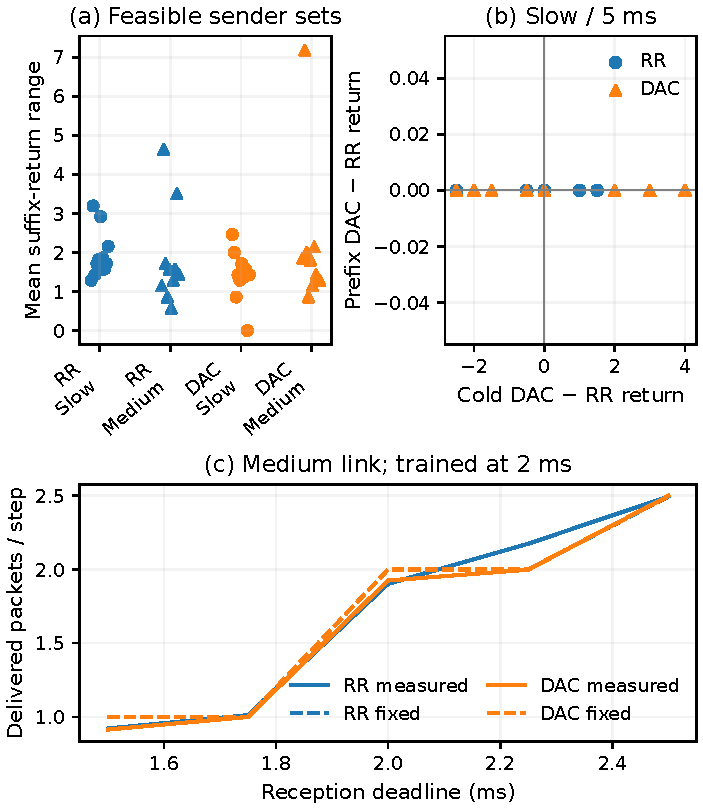
\includegraphics[width=\linewidth]{diagnostics.pdf}
\caption{Primary-checkpoint diagnostics. Left: each point is one seed's mean feasible-subset suffix-return range. Middle: Slow/5 ms only, cold and common-prefix DAC--RR effects on the same frozen policy, with early termination retained. Right: medium link, primary Medium/2 ms-trained RR/DAC checkpoints, mean delivered packets over ten seeds under measured (solid) or fixed (dashed) readiness. Seed-specific curves are retained in the supplementary summary; this panel shows means without uncertainty bands. These are distinct interventions, not pooled training cohorts.}\label{fig:controlled}
\end{figure*}
\subsection{A scheduler comparison also changes the history of reception}\label{sec:history}
TMC retains buffered messages between transmissions~\citep{zhang2020succinct}, and the restricted-bandwidth DIAL baseline in SchedNet reuses updates from unscheduled senders~\citep{kim2019schedule}. With this persistence, switching access at reset changes both the initial information acquired and later refreshes. We therefore branch after a common RR history, once every sender has a valid cache entry. The two branches inherit the same environment state, recurrent state, receiver cache, credit, sender ages and remaining horizon. Prefix costs are included; episodes terminating before the branch remain in episode averages with zero suffix contrast.

\paragraph{Switching after an identical history}
After the common RR prefix, suffix return changes in 0 of 400 Slow/5 ms episodes and 15 of 400 Medium/2 ms episodes. Early termination is retained (Supplementary Section~S3). In the slow condition, 126 pairs nevertheless differ in delivered sets and 94 in actions on common suffix steps. Of 373 survivors, 38 have no unresolved group, 296 have one and 39 have two, with nine steps remaining. An executed global-state action reference verifies unused attainable reward in 335/400 pairs. This reference changes actions and can exploit state unavailable to the deployed policies. Thus identical messages, universal termination and reward saturation do not explain the zero return contrast. The same finite-horizon return can thus hide different later information and actions, even when additional reward remains attainable.

\begin{table*}[pos=t]\centering\small
\caption{Changing the same access rule at different points in a trajectory. All differences are DAC minus RR with the indicated frozen weights and fixed readiness. Each row has ten training seeds and 20 paired resets per seed. The prefix comparison includes episodes that terminate before full sender coverage; its intervals use the ten seed means. Cold-start values are means.}\label{tab:history_by_cohort}
\begin{tabular}{llrrr}\toprule
Condition & Weights & Switch at reset & Switch after shared history [95\% CI] & Prefix survivors\\\midrule
Slow/5 ms & RR & $-0.850$ & $0.000$ [$0.000$, $0.000$] & 183/200\\
Slow/5 ms & DAC & $0.200$ & $0.000$ [$0.000$, $0.000$] & 190/200\\
Medium/2 ms & RR & $-1.700$ & $0.350$ [$-0.235$, $0.935$] & 199/200\\
Medium/2 ms & DAC & $-0.200$ & $-0.350$ [$-1.025$, $0.325$] & 200/200\\
\bottomrule\end{tabular}
\end{table*}

Table~\ref{tab:history_by_cohort} shows the comparison separately for the two weight sets. In Medium/2 ms, the shared-history means have opposite signs under RR-trained and DAC-trained weights, and both intervals include zero. Thus the full-episode contrast is not a stable estimate of a rule's effect after an arbitrary common history. The intervention inherits the policy's recurrent state and remaining task as well as its cache.

The remaining-opportunity reference helps interpret the zero slow-link contrast. It uses full environment state to schedule feasible group arrivals, and achieves its predicted suffix reward in executed trajectories. Of the 400 slow-link endpoints, 296 permit 10 additional reward and 39 permit 20; the remaining 65 permit none. The corresponding Medium counts are 260, 139 and one. Universal termination or exhausted reward opportunities therefore do not explain the small selector contrasts. The gap concerns what the frozen policies achieve after the communication intervention, even at states where a different action strategy could earn more.


The contrast depends on when the access rule is changed. Table~\ref{tab:which_switch} compares three ways of asking whether priority access helps in the same slow-link setting. Training and deploying under each rule measures the combined change in weights and access. Holding RR-trained weights fixed and switching at reset measures the change over an entire episode. Switching after the common prefix measures the remaining effect at the states reached by RR. The shrinking contrast follows a change in the intervention and the states at which it is applied. The common prefix matches the whole past trajectory, so a separate intervention is needed to identify an effect of receiver memory.

\begin{table*}[pos=t]\centering\small
\caption{What changes when priority replaces RR? Three existing Slow/5 ms comparisons, each with ten training seeds. The first row uses measured readiness and 50 resets per seed (paired bootstrap interval). The other rows use the same RR checkpoints, fixed readiness and 20 resets per seed. The shared-prefix row retains early terminations.}\label{tab:which_switch}
\begin{tabularx}{\textwidth}{@{}XXr@{}}
\toprule
Policy weights & Change to access & Mean priority minus RR return\\\midrule
Train independently under each rule & Deploy each policy under its training rule & $-1.40$ [$-3.06$, $0.08$]\\
Freeze the RR-trained policy & Switch at episode reset & $-0.85$\\
Freeze the same RR-trained policy & Switch after common RR history & $0.00$ in all 200 pairs\\
\bottomrule
\end{tabularx}
\end{table*}

\paragraph{Receiver memory changes actions at a flat reward endpoint}
The temporal-reuse mechanism in TMC~\citep{zhang2020succinct} makes cached information a plausible explanation. We test it directly at the shared-history endpoint.
A separate intervention crosses the two subsequent access rules with keeping the cache or clearing its payloads and validity timestamps at the same RR-prefix endpoint. We retain the environment state, recurrent state, receiver cache, credit, sender ages, cursor and remaining horizon before applying the memory intervention. In Slow/5 ms we replayed ten RR checkpoints on 20 resets each, keeping the 17 early terminations in the episode averages. The retained-cache branches reproduce the original suffixes. Clearing memory changed subsequent action histories in 154/200 RR and 155/200 DAC pairs. Every observed suffix return was zero in all four branches. A return-only comparison would miss a strong behavioral response to memory removal. Because suffix reward is zero throughout, this comparison cannot determine whether memory mediated the earlier return contrast. Matching a history and erasing a cache answer different questions; neither licenses assigning the whole scheduler difference to initialization.
\begin{table}[pos=t]\centering\small
\caption{Direct memory removal at the common Slow/5 ms RR-prefix endpoint: ten RR checkpoints and 200 resets, including 17 early terminations. All four retained/reset $\times$ RR/DAC branches have zero suffix return in every episode. Action differences compare cleared with retained memory under the same subsequent access rule.}\label{tab:memory_reset}
\begin{tabular}{lrr}\toprule
Later access & Changed histories & Changed returns\\\midrule
RR & 154/200 & 0/200\\
DAC & 155/200 & 0/200\\
\bottomrule\end{tabular}
\end{table}

Table~\ref{tab:memory_reset} makes the limitation of the reward endpoint explicit. The memory intervention has a large behavioral effect, while its selector interaction on return is identically zero in the observed sample. The privileged action reference and the memory reset answer complementary questions: the former tests whether reward remains attainable in the task, and the latter tests what these frozen policies do when their stored information is removed. A zero return effect cannot be read as unchanged behavior. Nor does matching a full history isolate cached information as the cause of the earlier return contrast.


\subsection{A shared link does not give selectors the same reception opportunity}\label{sec:timing}
DACOM makes waiting time part of the communication decision~\citep{yuan2023dacom}; joint computation and transfer models likewise charge work before an inference result is available~\citep{jung2023splitting}. In a sender comparison, preparation time consumes the same deadline as transmission. Matching bandwidth and offered caps therefore need not match reception opportunity. At Medium/2.25 ms, three 48-byte packets require readiness within 310 microseconds, after a 450-microsecond reserve, 50-microsecond propagation and 1.44 ms serialization. RR/DAC mean gate times are 128.7/208.4 microseconds; mean deliveries are 2.175/1.999 packets under measured readiness and 2.000/2.000 under fixed 500-microsecond readiness. Readiness tails and bookkeeping, not mean gate cost alone, determine service opportunities. Thus a nominally identical link does not present both implementations with identical reception opportunities.

\paragraph{Preparation cost persists across processes}
Three independent processes repeated the comparison on the same pinned CPU, using ten seeds and three resets per cell. At 2.25 ms, episode-weighted RR delivery means were 2.206, 2.005 and 2.002 packets per step, versus 2.000 in each repeat for DAC. The selector incurred extra computation on identical input snapshots in all three runs. Whether that overhead cost a reception opportunity depended on the timing and credit available on the individual step.

\paragraph{Preparation time and packet boundaries}
For a third packet on the Medium link, the preparation budget in microseconds is $D_{\max}-1{,}940$ with $D_{\max}$ expressed in microseconds. At deadlines of 2.00, 2.25 and 2.50 ms this leaves 60, 310 and 560 microseconds. In the original sweep, the percentages of decisions delivering a third packet under RR/DAC were 0/0, 17.5/0 and 49.3/49.8, respectively (average within episode, then within and across seeds). Credit also limits a third transmission. At 2.25 ms, RR's third-packet advantage varied across independent processes. Across identical-input snapshots, DAC added 98--100 microseconds to gate computation under episode-first weighting, with zero paired differences in delivered count on those snapshots. The extra cost changes delivery when it crosses a packet boundary on a step with enough credit. The persistent result is the extra selector work; its effect on packet reception depends on which side of the deadline boundary a step falls. A fixed-readiness comparison isolates sender choice, while measured readiness reveals the reception cost of implementing that choice.
\subsection{Informative reception does not ensure that the actor exploits it}\label{sec:receiver_decision}
\citet{lowe2019pitfalls} separate informative signaling from behavioral use. Supplementary Section~S4 applies that distinction after deadline-constrained delivery: we compare an unchanged acting policy with a probe of the aggregate it actually receives. Under source-aware selection, held-out decoding of the actual receiver aggregate reaches 99.91--100\%, while the unchanged policies achieve 64.17--78.44\%. The aggregate contains task-relevant information that the acting policy does not fully exploit. This is the post-reception ambiguity: changing access could supply more information without resolving the receiver's use of it. We first test the gap under normal access, then change the acting head. Supplementary Section~S4 gives the earlier probe protocol.
\paragraph{The use gap persists on the normal access distribution}
We used the ten Medium/2 ms broadcast RR checkpoints. The ideal-link reference had first passed the prespecified accuracy criterion in all ten seeds. On fresh evaluation resets under normal RR access, a linear decoder fitted on ten separate episodes could read the current bit from the aggregate with 69.37\% accuracy. The unchanged actors achieved 56.58\% on those same fresh resets, a paired gap of 12.79 percentage points (95\% seed interval 8.12--17.47). Normal RR supplied the current source update on 40\% of steps. Because each bit is independent of history and the RR schedule is independent of its value, expected follower accuracy on the remaining steps is one half. Even a perfect decoder on timely source updates therefore has expected accuracy at most $0.40+0.60/2=0.70$ in this regime. The gap therefore persists on the policy's normal access distribution and cannot be explained solely by privileged source selection.

\paragraph{Changing the actor tests the diagnosis}
We then fitted only the follower action head on the ten fit episodes using 100 full-batch supervised updates on 200 labelled bit observations (800 follower examples per seed and access rule), and evaluated its actions in fresh closed-loop rollouts (20 paired resets per seed). The source head, message encoder and scheduler parameters stayed fixed. A control received the same inputs and update budget with bit labels permuted across timesteps, keeping all four followers together. Fitting all 40 adapted and shuffled 4,930-parameter heads took 3.06 seconds on the study CPU. The rollout wrapper evaluates both heads for every treatment. Normal-access accuracy rose from 56.58\% to 63.01\%, a gain of 6.43 points [3.32, 9.54] over the unchanged head and 14.91 [10.04, 19.77] over the shuffled-label head. On the 20-step horizon this corresponds to 1.29 additional return points [0.66, 1.91]. One normal-access seed lost 1.19 points (Fig.~\ref{fig:adaptation}). These intervals average episodes within each of ten seeds and use an unadjusted paired $t$ interval. The admitted bytes (96 per step), delivered payload (64 bytes), sender identities and timestamps matched across heads. Later actions, including source actions, and message contents could change through feedback. The comparison measures the total effect of a limited supervised adaptation under the same access rule.

With source-aware access, accuracy rose from 65.08\% to 87.74\% (+22.67 points [13.28, 32.06]). This privileged intervention used a cloned selection state. Once its measured overhead and modeled waiting were charged, every source-aware step exceeded the 2 ms action deadline. Normal-access miss fractions were 1.63\% and 3.53\% for the original and adapted wrappers. These returns are measured at fixed packet readiness, without an extra reward penalty for late actions. The additional labels improve how the learned policy acts under this access schedule, while the higher miss rate prevents interpreting the reward gain as improved hard-deadline operation.

\begin{figure}[pos=t]\centering
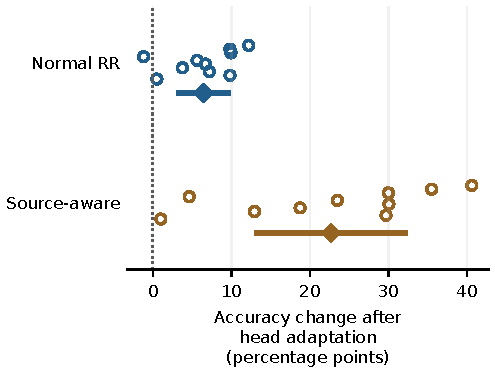
\includegraphics[width=\linewidth]{receiver_adaptation.pdf}
\caption{Change in acting accuracy on new broadcast episodes after fitting follower heads. Circles show each training seed's gain over the unchanged head, diamonds the ten-seed mean, and bars paired 95\% $t$ intervals. Normal RR supplies a current source update on 40\% of steps. Source-aware selection supplies it on all steps and incurs extra diagnostic CPU cost.}\label{fig:adaptation}
\end{figure}
\begin{table*}[pos=t]\centering\small
\caption{Receiver adaptation with a matched shuffled-label control. Each access regime uses ten seeds, ten fit episodes and 20 fresh evaluation episodes per arm and seed. Accuracy and deadline misses are seed means in percent. The unchanged-input probe is fitted on the separate fit episodes and evaluated on inputs from the unchanged actor. All acting arms retain the same admission schedule within each regime.}\label{tab:receiver_controls}
\begin{tabular}{llrr}\toprule
Access & Receiver & Accuracy (\%) & Action deadline misses (\%)\\\midrule
Normal RR & Unchanged & 56.58 & 1.63\\
Normal RR & True-label adaptation & 63.01 & 3.53\\
Normal RR & Shuffled-label adaptation & 48.10 & 2.05\\
Source-aware & Unchanged & 65.08 & 100.00\\
Source-aware & True-label adaptation & 87.74 & 100.00\\
Source-aware & Shuffled-label adaptation & 51.01 & 100.00\\\midrule
Normal RR & Probe of unchanged inputs & 69.37 & ---\\
Source-aware & Probe of unchanged inputs & 99.94 & ---\\
\bottomrule\end{tabular}
\end{table*}

The shuffled-label arm distinguishes the information in the fitting targets from merely applying extra optimizer updates (Table~\ref{tab:receiver_controls}). It uses the same inputs, architecture and 100-update budget, but breaks the relation between the current bit and its label. Its mean normal-access accuracy is 48.10\%, below the unchanged head's 56.58\%. The true-label head exceeds both controls. Thus the intervention converts task-relevant supervision into additional closed-loop reward on the tested policies; the probe alone had only established that the information was decodable.

The fixed access schedule also does not imply a fixed message stream after adaptation. Although encoder and source-head parameters stay unchanged, the source acts differently on 423 of 4,000 normal-access adapted steps and 409 of 4,000 source-aware adapted steps. Changed follower actions enter later recurrent inputs and can change later messages and source actions. The paired rollout therefore measures the total effect of the head update with feedback. This is why actual held-out episodes, rather than accuracy on the original frozen features, are needed to connect the receiver diagnosis to control.


The receiver intervention completes the distinction raised by the delivery tests. In MNIST-sum, the compared rules change which useful inputs arrive. In broadcast, labels help an acting head exploit information available under its existing access schedule, with later message contents free to change through feedback. Traffic and return alone do not locate this difference; observing the receiver input and then intervening on the actor does.

\section{Implications for Communication Evaluation}\label{sec:discussion}
The experiments expose successive ambiguities in the same inference. A reduction in offered traffic can remove only late attempts. Equal received counts can then hide different sender histories, and equal return can hide different actions. Even after sender identity is shown to matter, the factual priority may have no advantage over uniform feasible choices. Matching the whole preceding history changes the question again. Finally, timely information can remain underused by the acting receiver. Calling all of these outcomes ``communication efficiency'' is reasonable as a description of system cost and reward; assigning them all to useful message selection is not.

\begin{table*}[pos=t]\centering\small
\caption{Four stages for attributing a communication-efficiency result. Each comparison resolves a different ambiguity between offered traffic and control.}\label{tab:evaluation_protocol}
\begin{tabularx}{\textwidth}{@{}p{0.17\textwidth}XX@{}}
\toprule
Stage & Comparison needed & What the experiments establish\\\midrule
Validate learning & Compare channel access under matched training; intervene on messages for a frozen listener. Distinguish learned benefit from task necessity. & Hallway has a learned channel gap and an optimal local-clock solution. MNIST-sum shuffling reduces expected accuracy from 48.56\% to 9.78\%.\\[3pt]
Match delivery and cost & Pair weights, resets and cache rules; trace sender identities and timestamps. Compare measured with fixed readiness at the same link settings. & An 80\% offered-byte saving can preserve every action. Equal offered budgets can deliver different useful inputs; selector work can consume a reception slot.\\[3pt]
Isolate sender choice & Substitute feasible senders at fixed count and full state; compare with uniform choices. Match prior history and intervene separately on receiver memory. & Sender substitutions affect some states, but all four episode-weighted factual-minus-uniform intervals include zero. Cache removal changes actions even where suffix reward remains zero.\\[3pt]
Test receiver use & Probe the actual receiver input, then evaluate a changed acting head on fresh episodes at the same access schedule. & The normal-access decoder--actor gap leads to a supervised intervention that raises accuracy from 56.58\% to 63.01\%, with higher measured deadline misses.\\
\bottomrule\end{tabularx}
\end{table*}

For communication-reduction comparisons of the kind used by VBC and TMC~\citep{zhang2019efficient,zhang2020succinct}, a capacity-matched reference tests whether the claimed saving changes anything received. For access comparisons of the kind used by SchedNet~\citep{kim2019schedule}, a uniform feasible choice and a common-history branch test what a priority adds beyond channel access and prior information. For delay-aware control~\citep{yuan2023dacom}, preparation must be charged before counting usable packets. For signaling and listening diagnostics~\citep{lowe2019pitfalls,eccles2019biases}, a receiver intervention tests whether a measured information gap translates into additional reward. Table~\ref{tab:evaluation_protocol} puts these comparisons in the order needed to connect an offered message to control.

These distinctions change the interpretation of both positive and negative results. The Full--RR identity identifies a valid cost saving with no change in control. Nonzero sender sensitivity justifies investigating selection, but does not select a winning rule. The zero shared-prefix return contrast does not imply unchanged behavior or irrelevant memory. The supervised broadcast gain identifies one way to improve information use, with an observed deadline cost. Reporting the intervention and its paired effect keeps these conclusions separate while linking them to the same communication process.

\paragraph{Scope}
The experiments use Oracle-assisted five-agent Hallway, Oracle-free five-agent broadcast and a reconstruction of the one-step MNIST-sum game. The named literature supplies the comparisons and mechanisms examined; the measured effects are on the policies and channels specified here. MNIST-sum admission knows exogenous readiness and does not incur a prediction cost. Broadcast adaptation uses current-bit labels. Hallway branches require clonable full state, and enumerating alternatives takes $\binom{N}{k}$ suffix rollouts per state. CPU measurements cover one host. The transport model has serial service without losses, retries, backlog or compute/transfer overlap, and does not charge physical score-collection traffic. Late actions receive the environment's ordinary reward, so return and deadline compliance must be read separately.

The XOR reference failed its learning criterion in all ten seeds. An early SMACv2 pilot also failed; a later three-seed Terran campaign passed at 300,000 steps, but independent-engine replay failed at the second seed after 320 evaluation episodes. A separate one-checkpoint smoke verified delivery instrumentation over 20 episodes and 1,046 steps, including one 47-step Full--RR identity. It does not supply paired learned-policy effects across seeds. Supplementary Section~S5 records these outcomes. The present evidence establishes the ambiguities in the studied settings; their prevalence and magnitude in learned standard sequential benchmarks remain open.

\section{Conclusion}
Lower traffic and retained return establish a communication-cost outcome, but they do not explain what the selector contributed. Under deadlines, some offers can be removed without changing any received information; equal message counts can conceal different sender histories; and equal reward can conceal changed behavior. Feasible substitutions and shared-history interventions distinguish these cases from a benefit of the actual priority rule. Readiness measurements and receiver interventions locate two further sources of lost performance: information that arrives too late and information that the actor fails to exploit. Communication-efficiency evaluations become more informative when they connect the cost of an offer to its delivery, the history it changes and the response of the acting policy.

\section*{Data and code availability}
Code, trained checkpoints and evaluation outputs are included in the accompanying reviewer archive.

\FloatBarrier
\bibliographystyle{cas-model2-names}\bibliography{references}
\end{document}
